%%% Local Variables:
%%% mode: latex
%%% TeX-master: "../main"
%%% coding: utf-8
%%% End:
% !TEX TS-program = pdflatexmk
% !TEX encoding = UTF-8 Unicode
% !TEX root = ../main.tex

This section provides an overview of concrete applications and high-level procedures of 3D renderers. Furthermore, it introduces prior work conducted in this field, highlighting the novel aspects of this work. The goal is to show the potential and applicability of the developed solution. Details on the concepts and technologies involved will be introduced in \autoref{ch:theory} but may already be referenced briefly during the introduction.

\section{Use Cases}

The web is a versatile platform that can be used for various applications. Most consumer devices have access to a web browser, which makes it an ideal platform for reaching a broad audience. Compared to native applications, web applications have the advantage of being platform-independent and do not require installation. This facilitates the distribution of applications and reduces the barrier of entry for users.

E-commerce is a key use case for product renderings. Commonly, these applications rely on taking pictures of the product. Like traditional physical catalogues, this approach struggles with highly configurable products due to the amount of images required to cover all possible configurations. Computer graphics addresses this challenge through product configurators for virtual assembly and visualization. They alleviate the need for physical processes, such as photography, and are scalable to a large number of configurations. This can be implemented by creating 3D models of the components and assembling them in a virtual environment.

As the number of components grows and the product evolves, the marketing models used for end-user visualization need to be coordinated with product changes. To circumvent this issue, leveraging existing production \gls{CAD} models, prevalent in mechanical engineering and product design, offers a significant advantage. These models contain geometric and material information, which eliminates the need for redundant 3D models for marketing purposes. Geometric information defines the shape of the product, while material information refers to the surface description. One real-world example of a company with production \gls{CAD} data is EAO. They manufacture highly customizable industrial pushbuttons and operator panels. Due to the nature of the product, the number of possible assemblies grows exponentially with the number of component types.

To illustrate the use case in a simplified and universal form, consider a product assembled of $n$ component types. Each component type ($i$) has $o_i$ different options. This gives the total number of possible configurations ($t$) as shown in \autoref{eq:assemblyConfigurations}.

\begin{equation}
  t = \prod_{i=1}^n o_i
  \label{eq:assemblyConfigurations}
\end{equation}

For a product consisting of $n$ component types where each component type has the same amount of options ($o$), the equation can be simplified to $t = o^n$. This shows the exponential growth of possible assemblies.

One example at EAO is a specific product family within the so-called series 45. It has 14 component types ($n$), and each component type has approximately 10 different options ($o$). This results in $10^{14}$ possible configurations ($t$) based on 140 different components. In addition, EAO has many more product series and product families with varying numbers of components and options. This constitutes the primary use case considered for this thesis. The presented work uses EAO production models to demonstrate the feasibility and challenges of real-time rendering of highly configurable products. However, similar use cases can be found in other industries.

A web-based configurator using computer graphics for virtual assembly is well-suited to address such use cases where exponential growth in possible configurations is present.

\section{CAD Data Preprocessing}

To leverage production \gls{CAD} models, the models need to be preprocessed before they can be used for 3D rendering. The steps of such a pipeline, as used by EAO to show one possible variant, are visualized in \autoref{fig:cad-preprocessing}.

\begin{figure}[H]
  \centering
  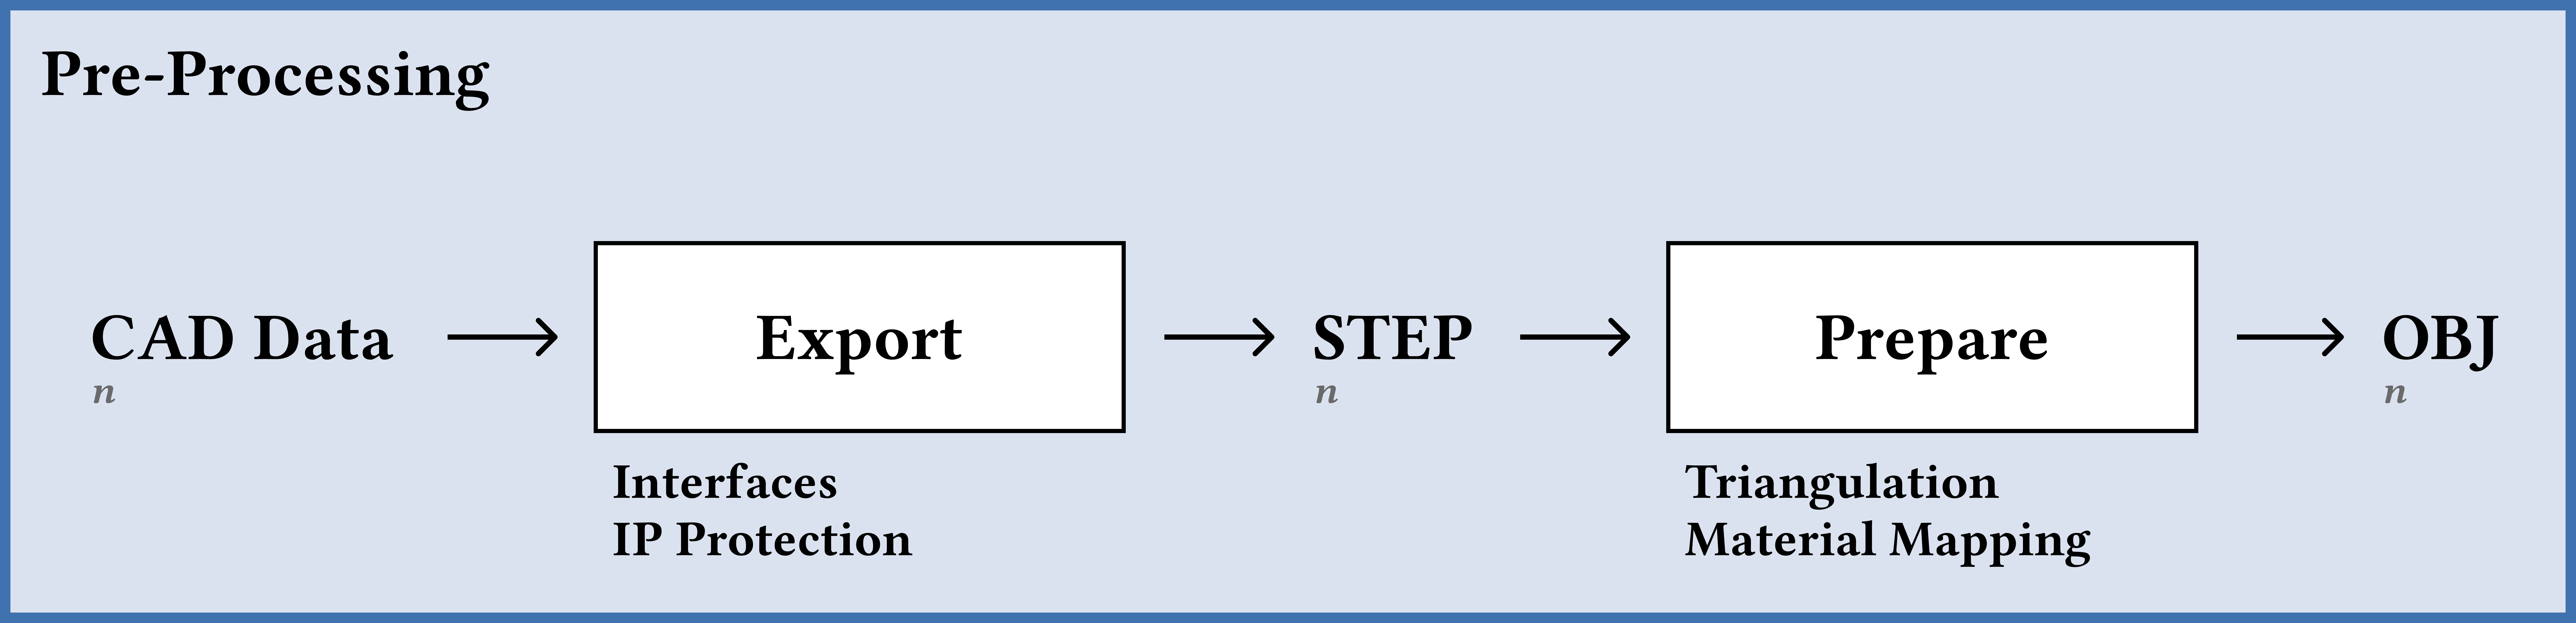
\includegraphics[width=0.9\columnwidth]{resources/cad-pipeline-preprocessing.png}
  \caption{A two-step preprocessing stage is employed for offline as well as real-time rendering pipelines.}
  \label{fig:cad-preprocessing}
\end{figure}

\fGls{STEP}{\e{Standard for the Exchange of Product model data}, a standard formalized in ISO 10303 for product manufacturing information.} files are a common format for exchanging \gls{CAD} data and can be used for this purpose. However, as will be discussed in \autoref{ch:specializedFormats}, other formats are more suitable for rendering and address the inherent limitations of \gls{STEP} files. An important consideration is intellectual property rights when using \gls{CAD} models from production processes. The models may contain proprietary information which should not be disclosed to the end user. As described by Stjepandić et al. \cite{ipr}, steps to circumvent this issue may include data filtering. Filtering can be implemented by removing meta information such as constraints or by removing occluded parts of the model, limiting the model to the hull of the assembly. As a positive side-effect, this potentially reduces the complexity of the model, which can be beneficial for rendering performance.

Preprocessing includes triangulation of the meshes, which is a common requirement for rendering engines. Frequently, the triangulated meshes are fine-grained and consist of a large number of triangles. This can lead to performance issues when rendering the scene. One way to handle this is to simplify the meshes by decimating triangles. Procedures for this purpose are well-established and include algorithms for generating level of detail (\gls{LOD}) artifacts \cite{luebke2003level}.

While numerous \gls{CAD} formats include material information, they are often unsuitable for rendering because they do not describe optical properties. To address this, a material mapping can be defined, translating \gls{CAD} materials to a suitable representation for the rendering pipeline. The concrete formats used for the preprocessing step are dependent on the \gls{CAD} software. However, conversion tools exist for most common \gls{CAD} formats and the general approach remains similar. After the preparation process, a rendering architecture paradigm can be employed to enable users to assemble the product virtually.

In addition, a rule set for the assembly must be defined. This rule set provides data on what component types can be added to the assembly and where they can be attached to. This interface definition can be provided using meta information files. Alternatively, this can also be represented geometrically within the model by using identifiable shapes to attach components to.

\section{Rendering Architecture Paradigms}

In order to render the assemblies based on the preprocessed information, three main paradigms can be employed for web-based applications: offline rendering, client-side real-time rendering, and remote real-time rendering. These paradigms differ significantly and the technology stack varies between them. Therefore, choosing a suitable paradigm is pivotal for the implementation of the application.

\subsection*{Offline Rendering}

Offline rendering requires pre-rendering all product configurations. This is theoretically possible for a finite number of configurations, but computationally expensive. 

An offline rendering pipeline generates static images of the assembly, which are then displayed in the browser. This means that all possible assemblies need to be rendered and stored upfront. As the number of component types increases, the number of possible combinations grows exponentially, which can lead to large amounts of storage and processing power being required, as shown in \autoref{fig:cad-offline}.

\begin{figure}[H]
  
\includegraphics[width=\columnwidth]{resources/cad-pipeline-offline.png}
  \caption{In an offline rendering setup, the number of images grows exponentially. The number of images increases further when offering 360° viewing.}
  \label{fig:cad-offline}
\end{figure}

Interactivity is limited by requiring all desired viewing angles to be defined upfront. 360° viewing experience using a single degree of freedom can be provided by rendering images in regular intervals. 100 images would be needed to get an image every 3.6°. These images can then be loaded in the browser as the user drags. However, if more degrees of freedom, different lighting situations, and zoom levels need to be supported, a similar growth in rendered images can be observed as for the assemblies.

In order to address latency, pre-loading images can be used. This may entail loading additional images in the background to enable a smooth user experience. However, this leads to increased bandwidth usage.

\subsection*{Client-Side Real-time Rendering}

An alternative to offline rendering is real-time rendering. For real-time rendering, client-side rendering is a frequently  used option. These approaches render the assemblies only as requested by the end user. This is the main benefit of using a real-time rendering pipeline, as illustrated in \autoref{fig:cad-online}. The rendering is done in the browser, limiting the server to serve the role of a file host and provide the geometry and material information in a 3D exchange format such as \fgls{glTF}{\e{Graphics Library Transmission Format, common 3D exchange format optimized for transmission and real-time rendering.}}. This approach is more flexible and can be used for a large number of configurations. The amount of data to be stored and processed offline grows linearly with the number of components, independent of the number of possible configurations.

\begin{figure}[H]
  
\includegraphics[width=\columnwidth]{resources/cad-pipeline-online.png}
  \caption{A real-time rendering pipeline solely relies on having an adequate model for each component of the assembly. It does not require pre-rendering every possible configuration.}
  \label{fig:cad-online}
\end{figure}

This approach limits the technology that can be used for rendering. The rendering is done in the browser, which means that it is dependent on the browser engine as well as the specific device hardware. It restricts the scene's complexity to the device's hardware constraints.

\subsection*{Remote Real-time Rendering}

For real-time rendering, an alternative paradigm is remote rendering \cite{remoteRendering}, which employs a server to render the scene and stream the visualization to the browser. The main drawbacks of this approach are network latency, reliance on network stability, and operational cost for the server infrastructure, which frequently requires dedicated \fGlspl{GPU}{\e{Graphics Processing Unit}, specialized processor for parallel computation} for rendering.

\begin{figure}[H]
  
\includegraphics[width=\columnwidth]{resources/cad-pipeline-remote.png}
  \caption{A remote rendering pipeline relies on a server to consistently stream the data in real-time to the client.}
  \label{fig:cad-remote}
\end{figure}

To fulfill thresholds frequently used for real-time rendering, the network latency should be below 20 ms. Recent studies have shown that this threshold is still a challenge, even when considering the fastest networks available at a given location. Many locations do not have access to any cloud data centers with a latency below 20 ms. \cite{cloudLatency}

\subsection*{Comparison}

A set of criteria is defined to evaluate the different paradigms. These criteria are used to show the advantages and disadvantages of each paradigm. The importance of each criterion is dependent on the specific use case and can be a primary determinant for the choice of paradigm.

\subsubsection{Preprocessing Cost}

Measure how much computation effort is required to prepare the data for rendering. Generally, lower is better. Offline rendering needs to pre-render all assemblies, essentially doing exhaustive rendering. Client-side rendering and remote rendering only need basic preprocessing.

\subsubsection{Hosting Cost}

The infrastructure cost involved in hosting the application during operations. Generally, lower is better. Offline rendering does not require application servers and mainly relies on storage for the generated images. Similarly, client-side rendering needs storage for the models. These two paradigms may employ \fglspl{CDN}{\e{Content Delivery Network}, distributed group of servers for caching content near end users.}. Remote rendering requires a rendering server. For scenarios where load is unpredictable, additional techniques such as auto-scaling and load balancing may be required. This can be costly and may induce additional complexity. In addition, bandwidth costs need to be considered.

\subsubsection{Storage}

The amount of data storage required for the application. Generally, lower is better. Offline rendering requires storage for all rendered images, possibly in multiple resolutions, to support different types of devices. Client-side rendering only requires storage for the models, as does remote rendering.

\subsubsection{Main Performance Dependency}

The main bottleneck in terms of rendering performance for the end user. Offline rendering sends static images, a process that is highly optimized by browser engines and image compression algorithms. Rendering such images is faster than real-time rendering, which is heavily dependent on the device hardware. Remote rendering is dependent on the network connection.

\subsubsection{Interactivity}

The level of interactivity the user can expect. Generally, higher gives more flexibility. Offline rendering means all possible views need to be pre-rendered. Extending views requires additional pre-rendering, which is optimally done using a delta change detection mechanism to prevent re-rendering unchanged views. Client-side rendering and remote rendering enable the user to interact in real-time without constraints. They also enable easier experimentation with different view configurations and open the possibility of using content provided by the end user in the rendering process. Such content could be lighting condition, background, or additional objects.

\subsubsection{Network Dependency}

The reliance on a stable network connection. Generally, lower is better. Offline rendering requires the loading of images, which is highly optimized in terms of data transmission and rendering performance. Client-side rendering requires an initial connection to download the models but is independent afterward. Remote rendering consistently requires a stable connection to stream the rendered images.

\subsubsection{Maximum Scene Complexity Dependency}

This determines the main bottleneck in terms of the complexity of the scene that can be rendered. Generally, using a server gives more flexibility as the provider has complete control over the hardware capabilities. Offline rendering can handle complex scenes given dedicated hardware. Client-side rendering is dependent on the device; the weakest supported device defines the possible scene complexity. Nowadays, rendering models with millions of triangles is possible on mid-range devices. Remote rendering can handle complex scenes, but is limited by the hardware constraints of real-time rendering, which does not cover huge scenes.

\subsubsection{Change Management Complexity}

This determines the ability to update the application based on new data. Generally, lower is better. Whenever a component changes, the application needs to be updated. Offline rendering necessitates re-rendering all images that contain the changed component. This can be a time-consuming process. Client-side rendering and remote rendering only require updating the model data and possibly meta information. This requires minimal changes in the application.

\subsection*{Assessment}
\label{ch:paradigmAssessment}

Each of the paradigms has its own advantages. \autoref{tab:paradigmComparison} highlights the strengths and weaknesses of each approach and provides a comparison of the criteria.

\begin{table}[H]
  \centering
  \ra{1.3}
  \begin{tabular}{@{}p{5cm}p{2.5cm}p{2.5cm}p{2.5cm}@{}}
  \toprule
  Rendering Paradigm & \textbf{Offline} & \multicolumn{2}{c}{\textbf{Real-time}} \\
   &  & \textbf{Client-Side} & \textbf{Remote} \\
  Preprocessing Cost & High & Low & Low \\
  Hosting Cost & Low & Low & High \\
  Storage & High & Low & Low \\
  Main Performance \newline Dependency & network & device & network \\
  Interactivity & Low & High & High \\
  Network Dependency & Low & Low & High \\
  Max Complexity Dependency & server & device & server \\
  Change Management \newline Complexity & High & Low & Low \\
  \bottomrule
  \end{tabular}
  \caption{High-level comparison between different rendering architecture paradigms.}
  \label{tab:paradigmComparison}
\end{table}

Offline rendering is suitable for applications where pregenerating all images is feasible and limited interactivity is acceptable. Real-time rendering, either client-side or remote, is a suitable choice for applications where the number of possible configurations is high and interactivity is important. The choice between client-side and remote rendering depends on the network infrastructure and the complexity of the scene.
Generally, client-side rendering setups can be extended to support remote rendering and offline rendering, while offline rendering setups, as well as remote rendering setups, are possibly not capable of client-side rendering due to technical constraints imposed by the available technology. Based on this assessment, this work focuses on client-side rendering, with the possibility of extending it to other paradigms in the future.

\section{Prior Work}

This section highlights related work for web-based client-side real-time rendering. A rough overview of the different approaches is given, but more detailed information on concepts, technology, strengths and weaknesses, and the benefits ray tracing provides over rasterization will be discussed in \autoref{ch:computerGraphics}.

Rasterization is a rendering technique that projects 3D scene geometry onto a 2D plane. The technique has been widely adopted in real-time rendering due to its efficiency. However, rasterization has limitations in achieving photorealism. Effects such as shadow casting and reflection do not require additional techniques.

Ray tracing is a powerful technique for rendering photorealistic scenes, which inherently supports effects such as shadow casting and reflection. Historically, ray tracing has been used in offline rendering due to its computational complexity. However, advancements in hardware have enabled real-time ray tracing in various domains.

\subsection*{Web-based Real-Time Renderers}

Different web-based real-time rasterizers exist. The main options include:

\begin{itemize}
  \item {\gls{Three.js}} \cite{threeJSWebsite} — most widely used web rendering engine.
  \item {\gls{Babylon.js}} \cite{babylonJSWebsite} — popular web rendering engine.
  \item {\gls{PlayCanvas}} \cite{playCanvasWebsite} — game engine for the web.
  \item {\gls{A-Frame}} \cite{aFrameWebsite} — web framework for building virtual reality experiences.
\end{itemize}

In addition, \gls{Unity}, a common game engine for desktop and mobile applications, also supports \fgls{WebGL}{\e{Web Graphics Library}, since 2011 the de-facto standard API for rendering 3D graphics on the web} \cite{unityWebGLCompatibility}.

These engines focus on rasterization techniques and are widely used for web-based applications. The focus of these engines lies in real-time rendering performance as used in games, advertising campaigns, virtual reality (VR), augmented reality (AR), medical imaging, scientific visualization, and educational applications. However, they lack support for ray tracing. 

\subsection*{Web Path Tracers}
\label{sec:web-path-tracers}

Path tracing is a specific ray tracing technique. The first experiments of using \gls{WebGL} for path tracing were implemented as early as 2010. One such example is the Google experiment demonstrating a Cornell Box \cite{goral1984modeling} with basic primitive shapes such as spheres and planes \cite{pathTracerWallace}.

Since then, various open-source implementations for the web have been developed, accompanied by related research efforts \cite{academicWebGLPathTracer, academicWebGLPathTracer2}. While closed-source options exist, this work focuses on open-source variants. The inherent advantages of open-source software lie in the possibility of inspecting and modifying the code, as well as in permissive license agreements, which often allow for free use in perpetuity. Consequently, closed-source alternatives are not considered in this context.

Notable open-source path tracers for the web include:

\begin{itemize}
  \item{\texttt{three-gpu-pathtracer}} \cite{ThreeJsPathTracerJohnson} — One of the most widely known path tracers for the web developed by Johnson. This path tracer is implemented as a \gls{Three.js} plugin and uses \gls{WebGL} for rendering.  It is bundled as a library and can be used to render scenes in the browser.
  \item{\texttt{Three.js PathTracer}} \cite{ThreeJsPathTracerLoftis} — Path tracer based on \gls{Three.js} developed by Loftis. This path tracer is also implemented as a \gls{Three.js} plugin and uses \gls{WebGL} for rendering. It does not provide a library but can serve as a basis for further development.
  \item{\texttt{dspbr-pt}} \cite{PathTracerDassault} — Path tracer by Dassault Systèmes implemented in \gls{WebGL}. It implements the Dassault Systèmes Enterprise PBR Shading Model (\gls{DSPBR}). However, the implementation has not been updated in recent years.
\end{itemize}

All of these path tracers are based on \gls{WebGL} and are either plugins for \gls{Three.js} or support \gls{Three.js} scene description. A more detailed comparison of these path tracers is provided in \autoref{sec:comparisonToPriorWork}.

\subsection*{WebGPU}

\gls{WebGPU} is a new web \fGls{API}{\e{Application Programming Interface}} that leverages the power of \glspl{GPU} and serves as a successor to \gls{WebGL}. Various applications of \gls{WebGPU} have been investigated in recent years. Examples include Dynamical.JS, a framework for visualizing graphs \cite{dotson2022dynamicaljs}; RenderCore, a research-oriented rendering engine \cite{Bohak_Kovalskyi_Linev_Mrak_Tadel_Strban_Tadel_Yagil_2024}; and demonstrations of how to use \gls{WebGPU} for client-side data aggregation \cite{kimmersdorfer2023webgpu}.

Research on the performance comparison between existing 3D engines and \gls{WebGPU} engines has been conducted as part of the development of FusionRender, which concluded that measurable performance gains can be achieved by using \gls{WebGPU}, but only when effectively leveraging its novel design principles \cite{fusionRenderWebGPU}. Similar findings have emerged from other independent studies, showing that \gls{WebGPU} can be faster than \gls{WebGL} \cite{webGPUWebGis, fransson2023performance, CHICKERUR2024919}.

\subsection*{Conclusion}

Work has been conducted in related fields; this includes research into the applicability of \gls{WebGPU} as well as writing web-based path tracers using \gls{WebGL}. However, the research suggests that no open-source path tracing library using \gls{WebGPU} has been developed. In light of these findings, \gls{WebGPU} presents a transformative opportunity. It is particularly well-suited for the development of a new real-time path tracing library for the web, which provides an alternative approach to existing rasterization-based rendering engines.
